\documentclass[12pt, letterpaper]{article}
\usepackage{graphicx}
\usepackage[margin=1in]{geometry}
\usepackage{amsmath, amssymb, amsthm, mathrsfs}
\usepackage{fancyhdr}
\usepackage{tikz}
\usepackage{enumerate}
\usepackage{cancel}
\usetikzlibrary{positioning}
\usepackage[utf8]{inputenc}
\usepackage{xcolor}
\usepackage{framed}
\title{HW 1.3}
\author{Your Name}
\date{\today}
\pagestyle{fancy}
\renewcommand{\headrulewidth}{0pt}
\renewcommand{\footrulewidth}{0pt}
\fancyhf{}
\rhead{
    Zack Abdirashid\\
    2/17/26 \\
    MATH 405
}
\rfoot{Page \thepage}
\begin{document}
\paragraph{\underline{2.1} \\ \\} 
\textbf{2.} \textbf{(a)} For which values $n$ does $K_{n}$, the complete graph on $n$ vertices, have an Euler cycle? \\ 
\begin{center}
* Euler cycle \ \Rightarrow \text{complete graph \underline{and} all vertices of even degree}
    \begin{framed}
        We know that in any complete graph $K_n$, the degree of every vertex is $n-1$. So, if $n$ is odd, $n-1$ will be even, and every vertex in $K_n$ will have even degree. $\therefore$ any odd integer $n$ will force $K_n$ to have an Euler cycle.
    \end{framed}
\end{center}
\textbf{(b)} Are there any $K_n$ that have Euler trails, but not Euler cycles?
\begin{center}
    \begin{framed}
        We know any odd integer $n$ guarantees an Euler cycle. Suppose we choose an even integer $n$. We know that the degree of every vertex in a $K_n$ will be $n-1$, which is odd. So, that means in any $K_n$ where $n$ is even \underline{and} $n > 2$, we will have more than $2$ vertices of odd degree. So, the only possible $K_n$ that has an Euler trail but not Euler cycles is $K_2$.
        
        \vspace{0.3cm}
        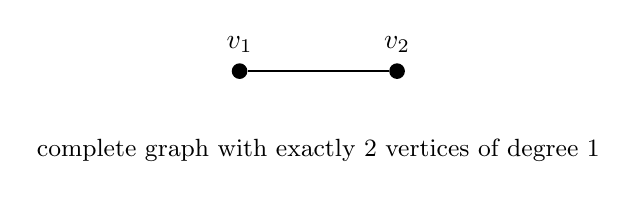
\begin{tikzpicture}
            \node[circle, fill=black, inner sep=2pt, label=above:$v_1$] (v1) at (0,0) {};
            \node[circle, fill=black, inner sep=2pt, label=above:$v_2$] (v2) at (2,0) {};
            \draw[thick] (v1) -- (v2);
            \node at (1,-1) {\small complete graph with exactly 2 vertices of degree 1};
        \end{tikzpicture}
    \end{framed}
\end{center}
\textbf{(c)} For which values of $r$ and $s$ does the complete bipartite graph $K_{r, s}$ have an Euler cycle?
\begin{center}
    \begin{framed}
        Since the degree of the vertices on the LHS of $K_{r,s}$ is $s$ and the degree of the vertices on the RHS is $r$, $r$ and $s$ must be even integers for every vertex in $K_{r,s}$ to have an even degree.
    \end{framed}
\end{center}
\vspace{0.3em}
\textbf{4.} What is the minimum number of times one must raise one's pencil in order to the draw the graph in Figure $1.4$?
\begin{center}
    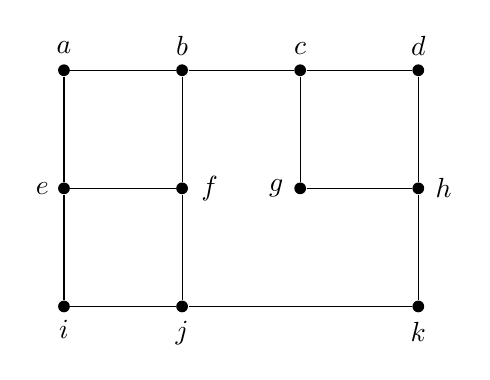
\begin{tikzpicture}[every node/.style={circle,fill,minimum size=1px,inner sep=1.5pt}]
    \node[label=90:$a$] (a) at (0,0) {};
    \node[label=90:$b$] (b) at (1.5,0) {};
    \node[label=90:$c$] (c) at (3,0) {};
    \node[label=90:$d$] (d) at (4.5,0) {};
    \node[label=180:$e$] (e) at (0,-1.5) {};
    \node[label=0:$f$] (f) at (1.5,-1.5) {};
    \node[label=180:$g$] (g) at (3,-1.5) {};
    \node[label=0:$h$] (h) at (4.5,-1.5) {};
    \node[label=270:$i$] (i) at (0,-3) {};
    \node[label=270:$j$] (j) at (1.5,-3) {};
    \node[label=270:$k$] (k) at (4.5,-3) {};
    
    \draw (a) -- (b);
    \draw (a) -- (e);
    \draw (b) -- (c);
    \draw (b) -- (f);
    \draw (c) -- (d);
    \draw (c) -- (g);
    \draw (d) -- (h);
    \draw (e) -- (f);
    \draw (e) -- (i);
    \draw (f) -- (j);
    \draw (g) -- (h);
    \draw (h) -- (k);
    \draw (i) -- (j);
    \draw (j) -- (k);
    \end{tikzpicture}
\end{center}
\begin{center}
    \begin{framed}
        To figure out the minimum number of times needed to raise your pencil to draw the above graph, we need to find the minimum number of Euler trails within the graph.\\ \\ 
        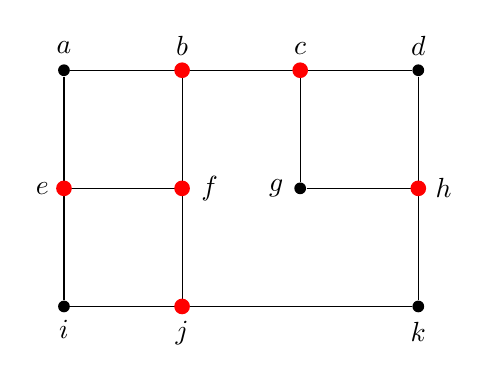
\begin{tikzpicture}[every node/.style={circle,fill,minimum size=1px,inner sep=1.5pt}]
    \node[label=90:$a$] (a) at (0,0) {};
    \node[label=90:$b$] (b) at (1.5,0) {};
    \node[label=90:$c$] (c) at (3,0) {};
    \node[label=90:$d$] (d) at (4.5,0) {};
    \node[label=180:$e$] (e) at (0,-1.5) {};
    \node[label=0:$f$] (f) at (1.5,-1.5) {};
    \node[label=180:$g$] (g) at (3,-1.5) {};
    \node[label=0:$h$] (h) at (4.5,-1.5) {};
    \node[label=270:$i$] (i) at (0,-3) {};
    \node[label=270:$j$] (j) at (1.5,-3) {};
    \node[label=270:$k$] (k) at (4.5,-3) {};
    
    \draw (a) -- (b);
    \draw (a) -- (e);
    \draw (b) -- (c);
    \draw (b) -- (f);
    \draw (c) -- (d);
    \draw (c) -- (g);
    \draw (d) -- (h);
    \draw (e) -- (f);
    \draw (e) -- (i);
    \draw (f) -- (j);
    \draw (g) -- (h);
    \draw (h) -- (k);
    \draw (i) -- (j);
    \draw (j) -- (k);

        \node[circle, fill=red, inner sep=2pt] at (0,-1.5) {};
        \node[circle, fill=red, inner sep=2pt] at (1.5,0) {};
        \node[circle, fill=red, inner sep=2pt] at (3,0) {};
        \node[circle, fill=red, inner sep=2pt] at (1.5,-1.5) {};
        \node[circle, fill=red, inner sep=2pt] at (4.5,-1.5) {};
        \node[circle, fill=red, inner sep=2pt] at (1.5, -3) {};
\end{tikzpicture} \\
However, we have more than $2$ vertices of odd degree: $b, c, e, f, h$ and $j$. So, adding $2$ imaginary edges to the graph,  \\
    \begin{tikzpicture}[every node/.style={circle,fill,minimum size=1px,inner sep=1.5pt}]
    \node[label=90:$a$] (a) at (0,0) {};
    \node[label=90:$b$] (b) at (1.5,0) {};
    \node[label=90:$c$] (c) at (3,0) {};
    \node[label=90:$d$] (d) at (4.5,0) {};
    \node[label=180:$e$] (e) at (0,-1.5) {};
    \node[label=0:$f$] (f) at (1.5,-1.5) {};
    \node[label=180:$g$] (g) at (3,-1.5) {};
    \node[label=0:$h$] (h) at (4.5,-1.5) {};
    \node[label=270:$i$] (i) at (0,-3) {};
    \node[label=270:$j$] (j) at (1.5,-3) {};
    \node[label=270:$k$] (k) at (4.5,-3) {};
    
    \draw (a) -- (b);
    \draw (a) -- (e);
    \draw (b) -- (c);
    \draw (b) -- (f);
    \draw (c) -- (d);
    \draw (c) -- (g);
    \draw (d) -- (h);
    \draw (e) -- (f);
    \draw (e) -- (i);
    \draw (f) -- (j);
    \draw (g) -- (h);
    \draw (h) -- (k);
    \draw (i) -- (j);
    \draw (j) -- (k);


        \node[circle, fill=red, inner sep=2pt] at (4.5,-1.5) {};
        \node[circle, fill=red, inner sep=2pt] at (1.5, -3) {};
    \draw[red, thick] (e) -- (b)
    \draw[red, thick] (f) -- (c)
\end{tikzpicture} \\
we now have exactly $2$ vertices of odd degree: $h$ and $j$. Since $2$ edges were added for this graph to have an Euler trail, one only needs to pick up their pencil \underline{$2$ times} to draw the graph. The sequence in which this is possible is as follows: \\ 
1) $c-g-h-d-c-b-a-e-i-j-f-e$ \\
2) $b-f-j-k-h$
    \end{framed}

\end{center}
\end{document}